\section{Luci}
\label{ch:luci}

\subsection{Structure}
\label{sec:luci:structure}
LC2 can be perceived as an IaaS provider, mediating between clients and *cloud* services for computational architecture analysis. Like most IaaS providers Luci's services fall into three different categories: ==storage==, ==networking== and ==computing==. We will broadly outline the main purpose of these functional units within the LC2 framework.

\subsection{Storage}
\label{sec:luci:structure:storage}
Luci provides functions to clients and services for storing network-wide data. However, compared to common IaaS storage systems, LC2 focusses on geospatial and geometric data. The storage is immutable, changes to the data are realized using **forward-incremental version control without synchronization** (?).

\subsection{Networking}
\label{sec:luci:structure:networking}
All communication in Luci is performed through a single broker, namely, the Luci server. Luci will validate the messages and, if valid, forward them to the designated service or client.

\subsection{Computing}
\label{sec:luci:structure:computing}
In the current state, service actions are delegated to a free computing service meeting the client-specified requirements. If there are no free computing services, the scheduler will [...]?

\subsection{Low-Level Protocol}

\begin{figure}[h!]
  \centering
  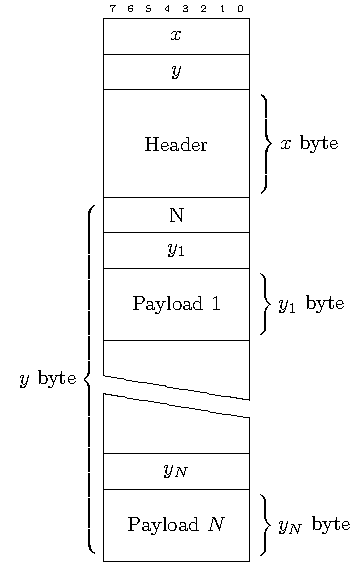
\includegraphics{bin/assets/binary-message-format.pdf}
  \caption{LC2 Message}
  \label{fig:lc2binary}
\end{figure}

\clearpage
